%%%% MACRO DEFINITION %%%%
% if any ...


%%%%%%%%%%%%%%%%%%%%%%%%%%%%%%%%%%%%%%%%%%%%%%%%%%%%%%%%%%%%%%%%%%%%%%%%%%%%%%%%%%%%%%%%%%%%%%%%%%%%%%%%%%%%%%%%%%%%%
%													BEGIN
%%%%%%%%%%%%%%%%%%%%%%%%%%%%%%%%%%%%%%%%%%%%%%%%%%%%%%%%%%%%%%%%%%%%%%%%%%%%%%%%%%%%%%%%%%%%%%%%%%%%%%%%%%%%%%%%%%%%%

\chapter{atomium --- The Python Structure Parser} % Write in your own chapter title
\label{Chapter3}
\lhead{Chapter 3. \emph{The Python Structure Parser}} % Write in your own chapter title to set the page header

%TC:macro \note [ignore]

\emph{Note that some of the material in this chapter has been published in the journal Bioinformatics under the title `atomium—a Python structure parser'.} \cite{ireland2020}

% write your code here
Much of this project relies very heavily on reading in structure data from files deposited in the Protein Data Bank.

Traditionally these files have been stored and distributed in the form of PDB (.pdb or .ent) files. These are text files that consist of a list of records, with each record being limited to 80 characters. Information is stored in these records at fixed offsets from the start of the line. This file format has a number of limitations, most notably the fact that they cannot store more than 100,000 atoms because only five characters are allocated to atom IDs, and so they cannot go past 99,999.

Consequently, the Protein Data Bank also provides files in the newer mmCIF (.cif) file format \cite{hall1991mmcif}, and indeed, structures with more than 100,000 atoms are \emph{only} available in this file format.

There are a number of parsers available that can handle these file formats, and which were considered for use in this project, both in Python and other languages. However, for reasons that will be outlined shortly, it was decided to create a novel Python parser. This parser is called atomium.

\section{Rationale}

The tool used to read structure files is of such critical importance to this project, that it was important to ensure that the correct tool with the correct \emph{capabilities} was used. Specifically, the tool would need the following properties:

\begin{itemize}
  \item The ability to read .cif files. Some structures are \emph{only} available in this form as they contain too many atoms to fit in a single .pdb file, so .pdb parsing alone would lead to an incomplete (though still very large) coverage of the available structures.
  \item The ability to generate biological assemblies from the raw, asymmetric unit coordinates of the file. As will be outlined below, the structure actually described by these files is often not entirely representative of biological reality, and certain transformations must be performed before analysis can be done.
  \item The ability to extract certain items of descriptive data from the files. In addition to the actual coordinates of the structures' atoms, the files also contain `meta' information about the file, details of the experiment that produced them and the species the molecules came from, quality information such as resolution, and sequence information not obtainable from the model itself (which often contain missing residues). This information was needed to annotate a local database.
\end{itemize}

Probably the major Python PDB parser at time of writing is BioPython. This is a multi-purpose bioinformatics library, with many modules for dealing with general biological data formats. One of these modules allows for parsing of PDB structure files, and is frequently used in Python analyses of protein structures. However, BioPython's PDB reader does not support the processing of Biological Assemblies --- it can only give the user the asymmetric unit as a model. As this project relies on having that functionality as a core part of the parsing process, this makes using BioPython difficult. It does meet the other requirements in that it can parse .cif files and read the metadata, but biological assembly generation is too crucial for the library to be considered.

It was therefore decided to create a novel Python library for handling biological structures, which would focus solely on structural models (BioPython has many other disparate functions). An additional advantage to doing this was that it gave a much greater insight into the structure of these files, and of structural biology concepts generally.

\section{Data Structures}

The object returned by the various parsing functions is a \texttt{File} object. This essentially represents the actual file object itself rather than its structural contents, and has the `metadata', descriptive attributes referred to above. Some key attributes are:

\begin{itemize}
  \item \texttt{code} The PDB identifier of the structure.
  \item \texttt{title} An overall description of the structure.
  \item \texttt{technique} The experimental procedure used to generate the data, such as X-Ray Diffraction, NMR, etc.
  \item \texttt{source\_organism} The organism that the molecules were originally derived from. Note that in cases where the file lists multiple species, only the first is used.
  \item \texttt{expression\_system} The organism that the molecules were actually expressed in. Again just the first is assigned to this property if there are multiple.
  \item \texttt{resolution} A measure of structure quality.
\end{itemize}

There are many others, and the full documentation (\url{https://atomium.bio}) lists them all.

The two most crucial attributes of the root \texttt{File} object are \texttt{model} and \texttt{models}. A \texttt{File} object has one or more \texttt{Model} objects, representing the actual structures themselves, and these are accessible via \texttt{models}. Because most files just contain a single model, the \texttt{model} attribute points to the first \texttt{Model} object as a convenience.

The must fundamental structural object is the \texttt{Atom}. All structures are ultimately amalgamations of atom objects arranged in space, and all higher structures are just collections of atoms. An \texttt{Atom} object has attributes for its Cartesian coordinates, its element, its unique numeric ID, its name, and various other pieces of information extractable from PDB structures. Even before they are grouped into structures, \texttt{Atom} objects can do various feats based on these simple properties. The mass of an atom can be determined from its element, its distance to or angle with some other atom can be determined using their locations, they can be translated and transformed through space, etc. All of these are performable using methods of the \texttt{Atom} object.

Ultimately though, structures are not modeled as mere clouds of atoms, they are grouped into various molecules and other higher order structures. In atomium, the two objects which are direct containers of atoms are \texttt{Residue} and \texttt{Ligand}; the former is used when the structure of which they are part is part of a chain, and the latter when it is not. They both have properties for their ID and name, and residues additionally have methods pointing to the next and previous residue in the chain they are part of.

They also both have an attribute which points to their atoms, but these are not stored using a Python built-in object type such as list or set. Instead they are stored in an atomium-specific object called a \texttt{StructureSet}, which is optimised for storing atomium structure objects. In many respects this works in a very similar way to an actual set, but internally the objects are stored as a Python dictionary, where the IDs are keys, and the values are lists of objects with that ID. This makes lookup by ID much faster than it would otherwise be which is absolutely crucial in large structures.

Residues themselves are stored in \texttt{Chain} objects. This implements the Python iterable tools, so they have a length, allow access to residues by index, and can be iterated through in \texttt{for} loops. They store their residues in a \texttt{StructureSet}, but they are returned as an ordered tuple.

Both \texttt{Chain} and \texttt{Ligand} inherit from the class \texttt{Molecule}, which in atomium means they are `top-level' structures as far as a model is concerned. That is, a model is a collection of chains and ligands. In fact a \texttt{Model} object is initialised by passing in chains and ligands, with the ligands then being divided into water and non-water ligands, as this is often an important distinction.

The relationship of the classes is outlined in Figure~\ref{fig:atomium-classes}.

Models, chains, residues and ligands all inherit from the class \texttt{AtomStructure}. This is an abstract base class that any atom-containing class can inherit from, and provides many useful functionalities using those atoms. It allows a structure's mass or charge to be determined by summing the masses or charges of the atoms, allows for translation or rotation of whole structures, the generation of atomic formulae using Python \texttt{Counter} objects, and RMSD (Root Mean Square Deviation --- a measure of how different two structures are in the layout and location of their atoms) comparisons with other structures. The full functionality is described in the atomium documentation.

\begin{figure}
\centering
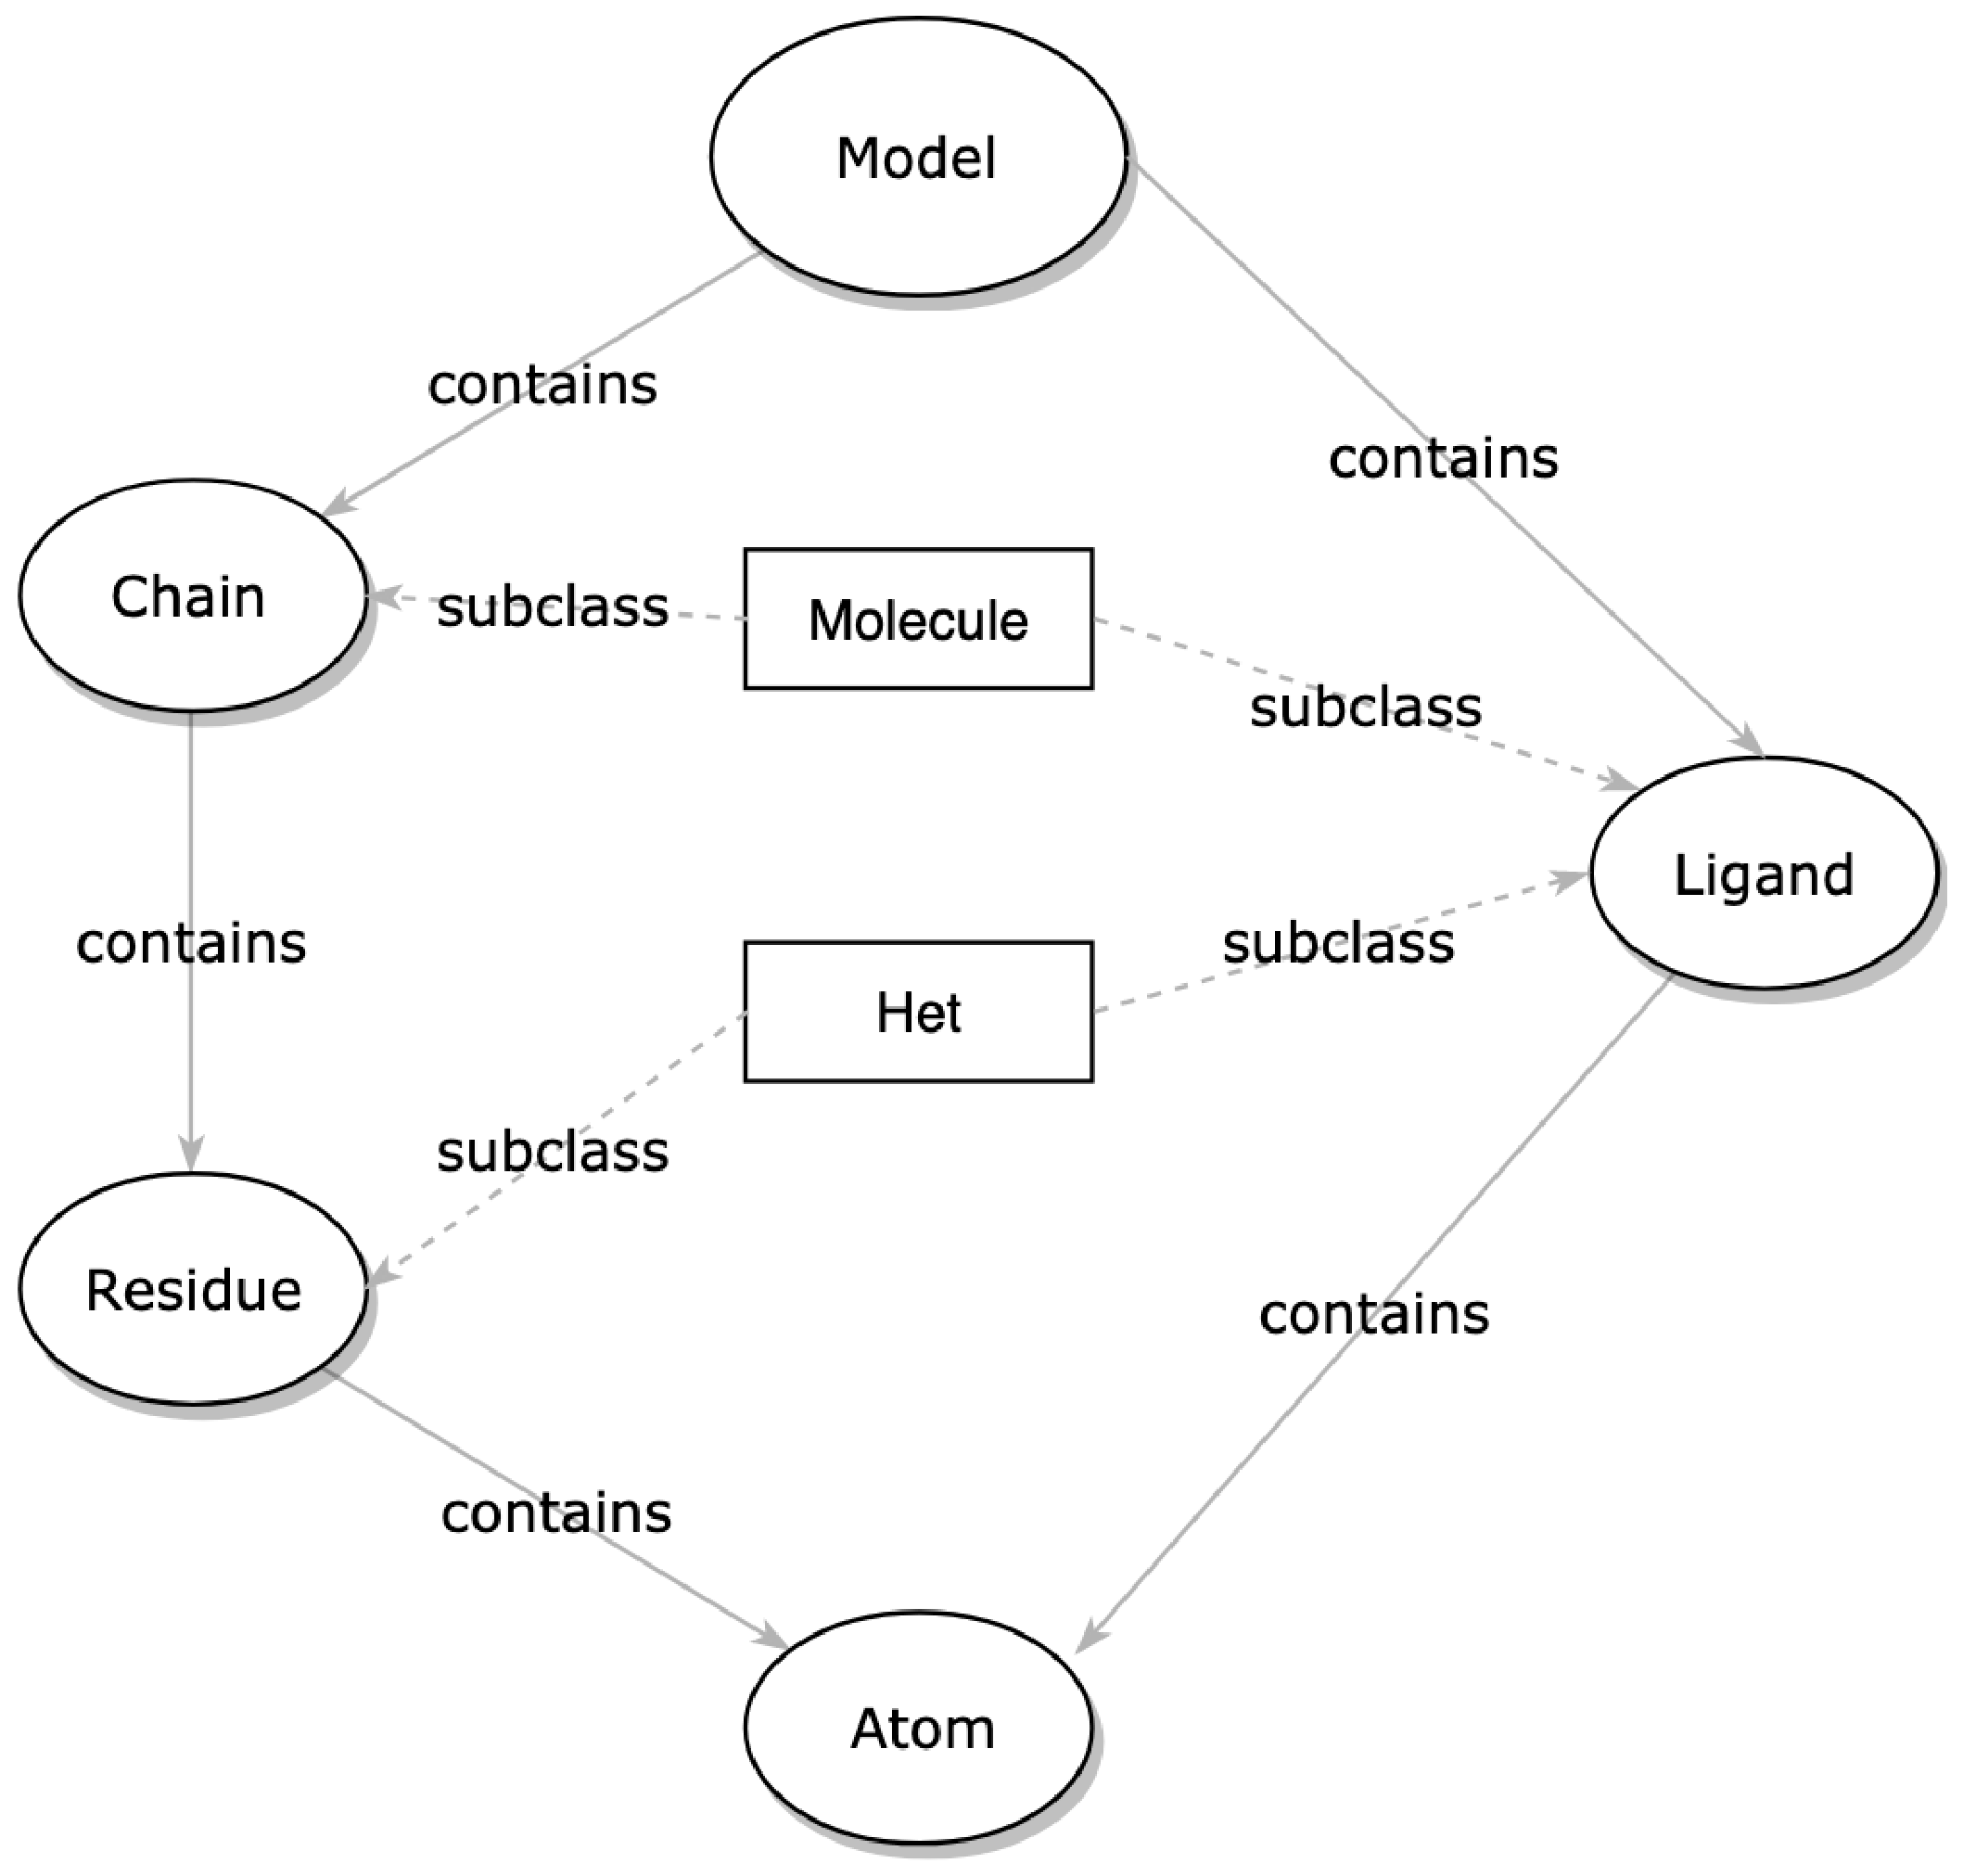
\includegraphics[width=1.0\textwidth]{Figures/atomium-classes.eps}
\caption[atomium classes.]{\label{fig:atomium-classes} The relationship of structure classes in atomium, representing the hierarchy of types. While the structures can be created from scratch, this hierarchy has been designed to reflect the hierarchy of object types in PDB and mmCIF files.}
\end{figure}

The structure classes also make use of an atomium metaclass called \texttt{StructureClass}. Essentially this confers on any object created from these classes, a set of lookup methods, allowing them to search the structures in their StructureSets by any property they might have, or any derivative of those properties. For example, chains can return any residues whose name matches a particular regex pattern, and models can return any atoms with a mass greater than some threshold. Earlier versions of atomuium had these properties manually coded in, but the current metaclass-based implementation ensures that all properties, all derivatives of properties, and any future properties can be instantly and rapidly searched (see Table~{table:filtering}.

These search functionalities all come in both single result (where a single structure or \texttt{None} is returned) and multiple result (where a set of results is returned, even if empty) versions.

\begin{table}
\begin{center}
\begin{tabular}{llr} \hline
Command                         & Result \\ \hline
\texttt{model.atoms()}                        & All atoms  \\
\texttt{model.atoms(element=`N')}                 & All nitrogen atoms \\
\texttt{model.atoms(mass\_\_gt=14)}                 & Atoms with mass greater than 14 \\
\texttt{model.atoms(name\_\_regex=`CA|CB')}             & CA and CB atoms  \\
\texttt{model.atoms(het\_\_name\_\_regex=`CYS|HIS')}    & Atoms in cysteine and histidine residues \\
\texttt{model.atoms(chain\_\_length\_\_lt=100)}     & Atoms in chains shorter than 100 residues \\ \hline
\end{tabular}
\end{center}
\caption{\label{tab:filtering}Examples of the filtering syntax that all atomium structures have by virtue of implementing the \texttt{StructureClass} metaclass.} 
\end{table}

Finally, all structures have an awareness of their context. That is to say, all atoms know which residue or ligand they are in, which model they are in, and so on, as do higher structures. This allows for neighbour searching. For example, atoms and higher structures can both look for atoms within a certain cutoff and which match certain criteria --- useful in, for example, a project that relies on identifying binding sites.

\subsection{Distance Optimisation}

While atomium is a general purpose PDB parser, some of its features are of particular significance to this project. An example of this is that of proximity detection, which allows atoms to identify nearby atoms within a cutoff. Higher structures can find nearby higher structures, but ultimately all of this is still relying on atoms searching for nearby atoms. As alluded to earlier, this is of particular importance in this project as a zinc atom's liganding atoms are determined by distance (and element). Any optimisation that can be done to this process is therefore important.

This process particularly needed optimisation as it is such a significant bottleneck in the generation of the dataset. To identify neartby atoms, an atom gets the full set of atoms in the containing model and iterates through them all, calculating the distance between that atom and itself. Those that fall below the given cutoff are returned. The algorithm which calculates distance is not particularly complex (it is just the Pythagorean equation extended to three dimensions) but when it is performed many times the burden can become considerable as the number of atom distances to calculate inreases with the square of the number of atoms in the structure for every proximity search. In large models with many thousands of atoms, finding an atom's nearby atoms means getting its distance to thousands of other atoms. For each metal atom in a structure, the metal's nearby atoms must be found, and for each binding site, each atom in each liganding residue must also find its nearby atoms to determine stabilising contacts in the secondary shell. Large structures also tend to have many binding sites, meaning that some PDBs would take more than a day to fully process.

\setlength{\emergencystretch}{1em}
To resolve this problem, atomium has been given the ability to speed up this process at the expense of greater memory consumption. An atomium model has an \texttt{optimise\_distances} method which, when called, organises the atoms into a grid. This is implemented using the Python \texttt{defaultdict} data structure, which is a mapping that creates a key if a new key is used, rather than throwing an error. These are nested three-deep so that each of the three dimensions is represented, and all the atoms in a single 10\AA\ cube are stored in one container. Once this grid is created, whenever at atom needs to search its neighbours, it uses its own location to work out which entries in the grid to look up using its own coordinates as keys, and then only searches these. The number of adjacent grid compartments to search is determined by the cutoff being used in the proximity search.

This optimisation can reduce the time taken to process a large PDB by three orders of magnitude.

\section{Parsing}

atomium can read .cif, .mmtf (a compact, stripped-down, binary representation of mmCIF files optimised for transmission over the web), or .pdb files. In each case the overall process is the same.

\begin{enumerate}
   \item Get the file contents as a string.
   \item Determine which filetype it is by looking at the file extension or, if not possible, by looking at file contents.
   \item Convert the filestring to a Python dictionary whose structure is specific to that file type.
   \item Convert that dictionary to a standard atomium data dictionary, whose structure is the same regardless of the file type origin.
   \item Convert that data dictionary to an atomium \texttt{File} object with one or more \texttt{File}s within it.
\end{enumerate}

This process for parsing has a number of advantages over just trying to go from filestring to processed Python object in one step. By making the parse process of the three filetypes converge at one data structure --- the atomium data dictionary --- it prevents duplication of effort involved in going from `data' to `Python structure'. It also means that every file can have a consistent, dictionary representations, which means that they can all be represented as JSON if desired. It is also easier for testing, as each stage in this (relatively complex) parsing process can more easily be tested in isolation.

\subsection{File Contents and File Type Detection}

Getting the file contents as a string is a straightforward process: it is simply opened and read using the built in Python functions for that purpose. The process is abstracted into a single function which will first try to read the file as a unicode string (appropriate for .cif and .pdb) and then as binary data (appropriate for .mmtf).

atomium also enables `fetching' a file from a remote server. Generally this is via HTTP, from the RCSB web servers \cite{burley2020pdb} with a four letter code, though the user can select any URL. The Python library requests \cite{requests} is used for this. Alternatively the user can fetch a file over SSH using a different atomium function.

Once the file contents are extracted as a string (or bytestring), atomium then determines which of the three file types it has been given, so it knows which functions to use to process it further. This is done using a straightforward algorithm: if the file extension is given, this will be used to determine filetype. If not, or if the filetype is not one of the three it recognises (such as .ent for example), atomium will assume it is .mmtf if the data is binary, .cif if it is a unicode string that contains the string \texttt{\_atom\_sites}, and .pdb otherwise.

The parsing time for the three file formats in atomium are of a similar order of magnitude, with .cif taking the longest (see Figure~\ref{fig:atomium-format-speed}). In all five cases, the relationship between the number of atoms and the time taken to parse is linear and, for all comparisons, care was taken to ensure the same kinds of parsing were being done—no biological assembly generation, proper relationship parsing and assigning for the sub-structures, etc.

\begin{figure}
\centering
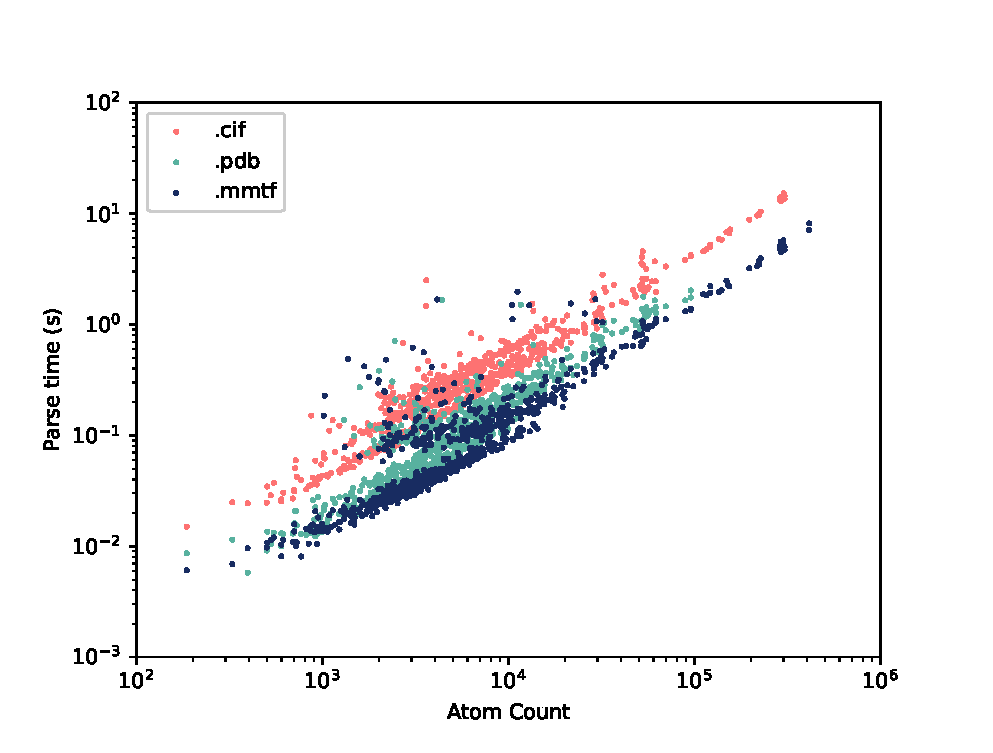
\includegraphics[width=1.0\textwidth]{Figures/atomium-format-speed.eps}
\caption[atomium parsing.]{\label{fig:atomium-format-speed} Time taken to parse the same 1000 randomly chosen single-model structures in the three file formats using atomium. Time as a function of atom count is linear and it can be seen that mmCIF structures take the longest, followed by PDB structures and MMTF structures.}
\end{figure}

\subsection{File Dictionaries}

The next step is to convert this string into a Python dictionary that reflects the internal structure of that file type.

.cif files are essentially a list of connected tables: tables in the sense that each block has a list of headers, and then one or more lists of values that belong to those headers, and connected in the sense that a row may have an ID as its first value which is refered to in another table. atomium represents these tables as lists of dictionaries, where the headers are keys, and the row cells the values. Each of these table lists is a value in the top-level dictionary. The main bottleneck in this process is splitting values on a single line --- they are white-space separated, albeit with whitepsace within quotes ignored, and with both quote types permissable and escapable within the other. Initially the Python library shlex was used to do this splitting, but its speed was just too slow so a custom function was written which was faster, though still the slowest part of the process.

.mmtf files are binary encoded Python dictionaries, so once the Python msgpack library has decoded it, it is essentially already in dictionary form. The only extra steps that need to be taken are to decode the .mmtf formatted binary fields within this dictionary, using the algorithms specified in the .mmtf documentation and implemented in atomium.

.pdb files have much less internal structure than the other two, and are essentially just lists of records. These records can be grouped by record name however, and this is what atomium does. The file dictionary has record names as keys, and lists of records that belong to that record type as values. The only exceptions are \texttt{REMARK} records, which are further grouped by remark number, and all model related records (\texttt{ATOM}, \texttt{TER}, \texttt{HETATM} etc.), which are grouped together because their order relative to each other is information that would be lost of they were split up into record types (\texttt{TER} records separating chains being the main reason).

This resultant file dictionary, whose internal structure is specific to file type, is essentially just a Python representation of the file contents --- no `parsing' is done as such, it just gets the information in a form that later processes can understand.

\subsection{Data Dictionary}

This file dictionary is then turned into an atomium `data dictionary'. This is a dictionary with a consistent internal structure regardless of what the original file type was, and essentially consists of a number of sub-dictionaries.

For example there is the description sub-dictionary, which contains meta information about the file such as title and deposition date. There is an experiment sub-dictionary, with information about how the model was created. The quality sub-dictionary contains resolution and other related information. The geometry sub-dictionary contains transformation matrices, such as those needed to create biological assemblies.

The most important one is `models', which is actually a list of sub-dictionaries. Each one contains informations about the chains, ligands and water molecules in that model, containing all the information needed to create an atomium \texttt{Model}.

Each of the three file dictionaries have their own functions for extracting information from them and building a data dictionary. In the case of .cif and .mmtf file dictionaries, this is relatively straightforward, as much of the data has already been extracted in the previous step, and this is largely just a question of transfering data from one dictionary to another, and nesting atoms within the right structures.

For .pdb files however, the previous step just grouped records, and the data is still locked away within these strings at pre-defined offsets, so for this filetype it is this stage which is the bottleneck, as it takes longer to extract the necessary information.

The parsing process is summarised in Figure~\ref{fig:atomium-parsing}.

\subsection{Model Generation}

The structure of the data dictionary is optimised to make model creation as rapid as possible. The polymers, ligands and water molecules are already segregated as they will be in the model, and all names and IDs are already parsed. Relevant \texttt{Model}, \texttt{Chain}, \texttt{Ligand} etc. molecules are created from this information.

The surrounding \texttt{File} object is made from the rest of the data dictionary with the meta information, with the values of the sub-dictionaries becoming properties of that object. The \texttt{Model} objects exist as a list within that \texttt{File}, with a pointer to the first \texttt{Model} if the user only needs the first.

Biological assemblies can be created using a \texttt{generate\_assembly} fuction. In earlier versions of atomium, each individual molecule was transformed separately, but in very large structures this can be time consuming. Instead, the copies are created, and then the atoms of all the structures are transformed in one step.

\begin{figure}
\centering
\includegraphics[width=1.0\textwidth]{Figures/atomium-parsing.eps}
\caption[atomium parsing.]{\label{fig:atomium-parsing} An overview of how parsing of the three file types is done. Because the three file types converge on a single data dictionary, all three file types can be represented as JSON.}
\end{figure}

\section{Saving}

One of the more unusual features of atomium is that it allows changes to models to be made and then for those changes to be saved in \emph{any} of the three file types that atomium supports.

Unlike the process of parsing, in which the structures pass through a number of different representations reflecting the different layers of abstraction of that process, saving is much more starightforward. A function takes in an atomium \texttt{AtomStructure} (it does not need to be a model --- chains etc. can be saved individually) and turns it into the relevant filestring.

Only structural information is saved. The various file annotations that are parsed from the original files are presumed to be properties solely of those original files, and not of any modified versions of them that might exist. So, atom records are saved, along with anything else needed to construct details of the actual structure model, but not titles, deposition dates, resolution etc.

\section{pdb2json}

As already noted, the process of parsing a structure file involves turning the raw filestring (or bytestring) into two successive Python dictionaries, before then being turned into a Python object. Initially this choice of Python dictionary as internal representation was a decision made to make development easier.

However, Python dictionaries have a structure very similar to JSON, a data format that is frequently used for sending data over the web in a very human readable way, as it is essentially just nested key-value pairs. Therefore, atomium is also potentially a tool for turning any PDB structure into JSON, if the data dictionary were simply converted to JSON using Python's built-in \texttt{json} library.

To this end, pdb2json was created. This is a simple, lightweight Django web app which uses atomium to take any PDB code and return the resultant structure as JSON. This is done using a URL - \texttt{/2SOD/} will return the JSON for the PDB 2SOD, for example.

It is currently available at \texttt{https://pdb2json.samireland.com/}.

By default, pdb2json tells atomium to use the .cif representation for parsing, but this can be altered using, for example, \texttt{/2SOD.pdb/}. The structure of the JSON returned will be the same, as atomium creates the same data dictionary regardless of file type, but some values might be different. For example, many PDBs have titles etc. in ALL CAPS whereas .cif files use title case, and atom IDs may be numbered slightly different. Generally the actual semantic content should be the same across all file types though.

If the user so wishes, they can get the initial Python dictionary as JSON (the one that is specific to that file type) using \texttt{/2SOD/?file} notation. This is generally of limited interest in the case of .pdb and .mmtf, except as a means of checking the original file contents pre-processing, but in the case of .cif it can be very useful. This is because \emph{every} attribute of the structure will be accessible in this dictionary, so if the subset of attributes atomium pulls out of files to annotate its final representation isn't enough, they can be obtained from this representation. For example, atomium File objects have \texttt{rvalue} and \texttt{rwork} attributes, but there are many supporting metrics for these calculations in the original file.

Obviously, PDB structures can be quite large, with some containing hundreds of thousands of atoms. The user may not wish to download the JSON for an entire structure when they only need a single metric or set of metrics. Therefore, pdb2json allows the user to traverse the keys of the JSON structure using the supplied URL. For example, while \texttt{/2SOD/} will return the JSON for the entire structure, \texttt{/2SOD/quality/} will return only the \texttt{quality} sub-dictionary that was part of the original JSON object. This traversal can be as deep as the user wishes: \texttt{/2SOD/models/0/non-polymer/O.153/atoms/4382} will return information about a single zinc atom, for example.

Note however that while this will reduce the volume of data that will be sent over the network, on the server the structure is still being fully processed. So this feature can save on bandwidth, but not really on request speed.

pdb2json then, is a lightweight web server for providing users with JSON representations of any PDB structure, acting as a thin wrapper around atomium. It was not necessary to the overall project or even to atomium itself, but it was felt the ratio of work needed to benefit provided to the wider community was so low that it would be a useful exercise to create. It means that researchers no longer require a PDB parser installed to get basic structural information --- just an HTTP client, such as a browser. It is language agnostic; most programming languages will have JSON libraries as part of their standard library, whereas PDB processing libraries like atomium or BioPython are much more specialised pieces of software. It also means that all structures now have a much more human readable format that is easily viewable.

%%%%%%%%%%%% END %%%%%%%%%%%%
